\section{O DEMO}
\subsection{Rozdíl mezi notací a metodologií}
V celém textu této diplomové práce se vyskytují dva jevy. O BPMN mluvíme jako o \textit{notaci} a o DEMO jako o \textit{metodologii}. Takto tyto techniky označujeme záměrně a myslím, že je na tomto místě účelné si vysvětlit rozdíl mezi pojmy \textit{notace} a \textit{metodologie}. Pochopení této odlišnosti totiž vnáší trochu světla k lepšímu pochopení rozdílu mezi BPMN a DEMO.

\subsubsection{Notace}
Notace označuje \textit{formální prostředky} pro popis reality. Například právě v oblasti analýzy a modelování podnikových procesů je notací sada grafických objektů, které pak používáme pro popsání samotného procesu. Na notaci je obvykle navázána související metodika. \cite{Notace}

Metodikou nazýváme \textit{popis pracovního postupu} nějaké činnosti, který je více či méně formalizovaný \cite{Metodika}. V případě modelovací techniky by taková metodika tedy popisovala jak při modelování postupovat a jak a kdy jednotlivé elementy přesně používat. To však v případě BPMN neplatí, jelikož BPMN není svázané s žádnou metodikou \cite{Vasicek2008} a tedy pokud se někde vyskytuje označení BPMN jako metodiky, je takové označení chybné.

\subsubsection{Metodologie}
Metodologie je oproti tomu vědní disciplína, která se zabývá tvorbou metod a jejich aplikací. Metodologie vědy je tedy naukou o metodách. Jak píše \cite{Ochrana2009} je teorií k výběru výzkumných metod a návodem, jak vybrané metody (metodu) používat ve vědeckém zkoumání.

Pod vlivem angličtiny se však i v češtině často setkáváme s tím, že pojmy metodika a metodologie splývají a jsou časfo zaměňovány. Můžeme nicméně vidět, že rozdíl BPMN a DEMO je na první pohled zřejmý v tom, že notace BPMN nemá za sebou zdaleka tak robustní základ jako metodologie DEMO. Tento fakt má několik důsledků týkajících se přístupnosti a přímočarosti použití obou technik. Tyto důsledky budou ještě v této práci dále rozebrány.

\subsection{Motivace k vytvoření DEMO}
Jak shrnuje \cite{Vejrazkova2013}, u základní úvahy tvůrců DEMO byl současný stav podniků a organizací, které jsou velmi komplexní a z toho důvodu je velmi obtížné mít pomocí současných nástrojů jasnou představu o tom, jak přesně fungují a co se v nich děje.

Moderní organizace jsou totiž založeny na propojení sociálních a technických komponent, které spolu vzájemně komunikují. Komunikace je tedy nejdůležitějším aspektem celé metodologie DEMO. Dle \cite{Dietz2006} je ontologie podniků (\textit{Enterprise ontology}) nejvhodnějším prostředkem k pochopení konstrukce a operací v podniku.

\begin{quote}
DEMO bylo vytvořeno jako metodologie pro vytváření ontologického modelu podniku. \cite{Vejrazkova2012}
\footnote{DEMO was developed to be a methodology for creating an ontological model of an enterprise. \cite{Vejrazkova2012}}
\end{quote}

\section{Ontologie}

V úplně základním pojetí je ontologie definována jako \textit{nauka o bytí.} Taková definice je samozřejmě pro čtenáře velmi abstraktní. Lepší by bylo ontologii definovat jako nauku o Bytí, tedy s velkým B, neboť ontologie se právě zabývá \uv{pouze} tím, co to znamená, že něco \uv{je}, jak to bytí vypadá a jak to funguje.

\begin{quote}
Ontologie (nebo ontologický model) organizace je definován jako porozumění chodu organizace, které je kompletně oproštěné od realizace a implementace vlastních činností.
\footnote{The ontology (or ontological model) of an enterprise is defined as an understanding of its operation, that is completely independent of the realization and the implementation of the enterprise. \cite{Dietz2005}}
\end{quote}

Pro lepší pochopení toho, co ontologický model představuje je užitečné uvést rozdíl mezi \textit{teleologickým} pojetím systému a \textit{ontologickým} modelem systému.

Teleologický pohled na systém se zabývá funkcemi a službami, které systém poskytuje navenek. Teleologický model pak vypadá jako tzv. \uv{black-box model} neboli vidíte, že se vstupy změní na nějaké výstupy, ale už není vidět, jak k tomu došlo. Tento pohled (model) je vhodný pro užívání a řízení (věcí, systémů, organizací).

Ontologický pohled se naopak zabývá tím, jak systém funguje uvnitř, tedy tím, \textit{jak} dojde k proměně vstupů na výstupy. Zabývá se tedy konstrukcí a chodem systému. Ontologický model je tedy typem tzv. \uv{white-box modelu}. Ontologický model najde uplatnění při budování a úpravách (věcí, systémů, organizací).

\subsection{Motivace pro zabývání se ontologiemi v organizaci}
Jak už bylo popsáno výše, ontologie v organizaci slouží zejména k porozumění jejímu chodu bez nutnosti zabývat se, jak jsou jednotlivé činnosti implementovány. Takový přístup je užitečný pro následující skupiny uživatelů: \cite{Dietz2005}

\begin{itemize}
\item \textbf{Manažeři} – Pro řízení větších celků je užitečné mít možnost oprostit se od detailů a dokázat se na chod takového celku podívat z vyšší perspektivy, tzv. \uv{big picture pohled}.
\item \textbf{Návrháři, inženýři, architekti} – Pro účely návrhu a úprav fungování chodu organizace je důležité mít podnikové procesy definované metodicky a nezávisle na jejich implementaci.
\item \textbf{Uživatelé} – Existují skupiny uživatelů (uvnitř i vně organizace), pro které je užitečné mít vhled i do fungování organizace nebo jejího celku.
\end{itemize}

\section{Teorie PSI (\ptheory)}

\begin{quote}
Teorie PSI neboli \ptheory{}  je teorie o fungování organizací. \cite{Dietz2005}
\footnote{The \ptheory{} is a theory about the operation of organizations. \cite{Dietz2005}}
\end{quote}

Zkratka PSI znamená \textit{Performance in Social Interaction}. Paradigma, na kterém je tato teorie založena říká, že subjekty, kterými jsou lidé v organizaci, vstupují do závazků a dodržují je. Tímto způsobem pak vzniká spolupráce mezi lidmi. 

Cílem \ptheory{} je umožnit porozumění funkcím
organizace bez vlivu toho, jak jsou tyto funkce ve skutečnosti operativně vykonávány. Jak uvádí \cite{Vejrazkova2013}, stejné cíle si klade i metodologie DEMO, takže je jen logické, že je právě na \ptheory{} postavena. Porozumění této teorii je tedy nezbytné pro správné pochopení a používání DEMO.

Teorie PSI se skládá ze čtyř axiomů:například

\begin{enumerate}
\item operační,
\item transakční,
\item kompoziční,
\item distinkční.
\end{enumerate}

\subsection{Operační axiom – The operation axiom} \label{sec:operacni_axiom}
První axiom \ptheory{} se nazývá \textit{operační}. Jeho základem jsou dvě tvrzení: \cite{Dietz2006}:

\begin{enumerate}
\item Chod organizace se skládá z aktivit, které vykonávají actoři. Actoři jsou kombinací \textit{zodpovědnosti} a \textit{autority} k provádění dané aktivity.
\item Při tom provádějí dva druhy činností: \textit{coordination a production acts (C-acts a P-acts)}. Výsledkem těchto činností jsou \textit{coordination a production facts (C-facts a P-facts)}.
\end{enumerate}

Provádět P-acty a P-facty znamená přivádět na svět něco nového a přispívat tak k podnikovým funkcím nebo službám. P-facty mohou být hmotné i nehmotné. Příkladem těch hmotných může být například vyrobení pizzy, příkladem nehmotných zase například vynesení rozsudku soudem.

Provádět C-acty a C-facty znamená, že actoři jednají v souladu se závazky, které se týkají tvorby P-factů. Zjednodušeně řečeno se jedná o \textit{komunikaci} ohledně vytváření P-factů.

Kromě C-factů a P-factů rozlišujeme ještě C-world a P-world. C-world je množina C-factů a stejně tak P-world je množina P-factů. Oba světy jsou tedy množinou factů, které byly vytvořeny do konkrétního momentu v čase. Vztah všech základních stavebních kamenů operačního axiomu je graficky znázorněn na obrázku \ref{fig:operation_axiom}.

\begin{center}
\begin{figure}[H]
\centerline{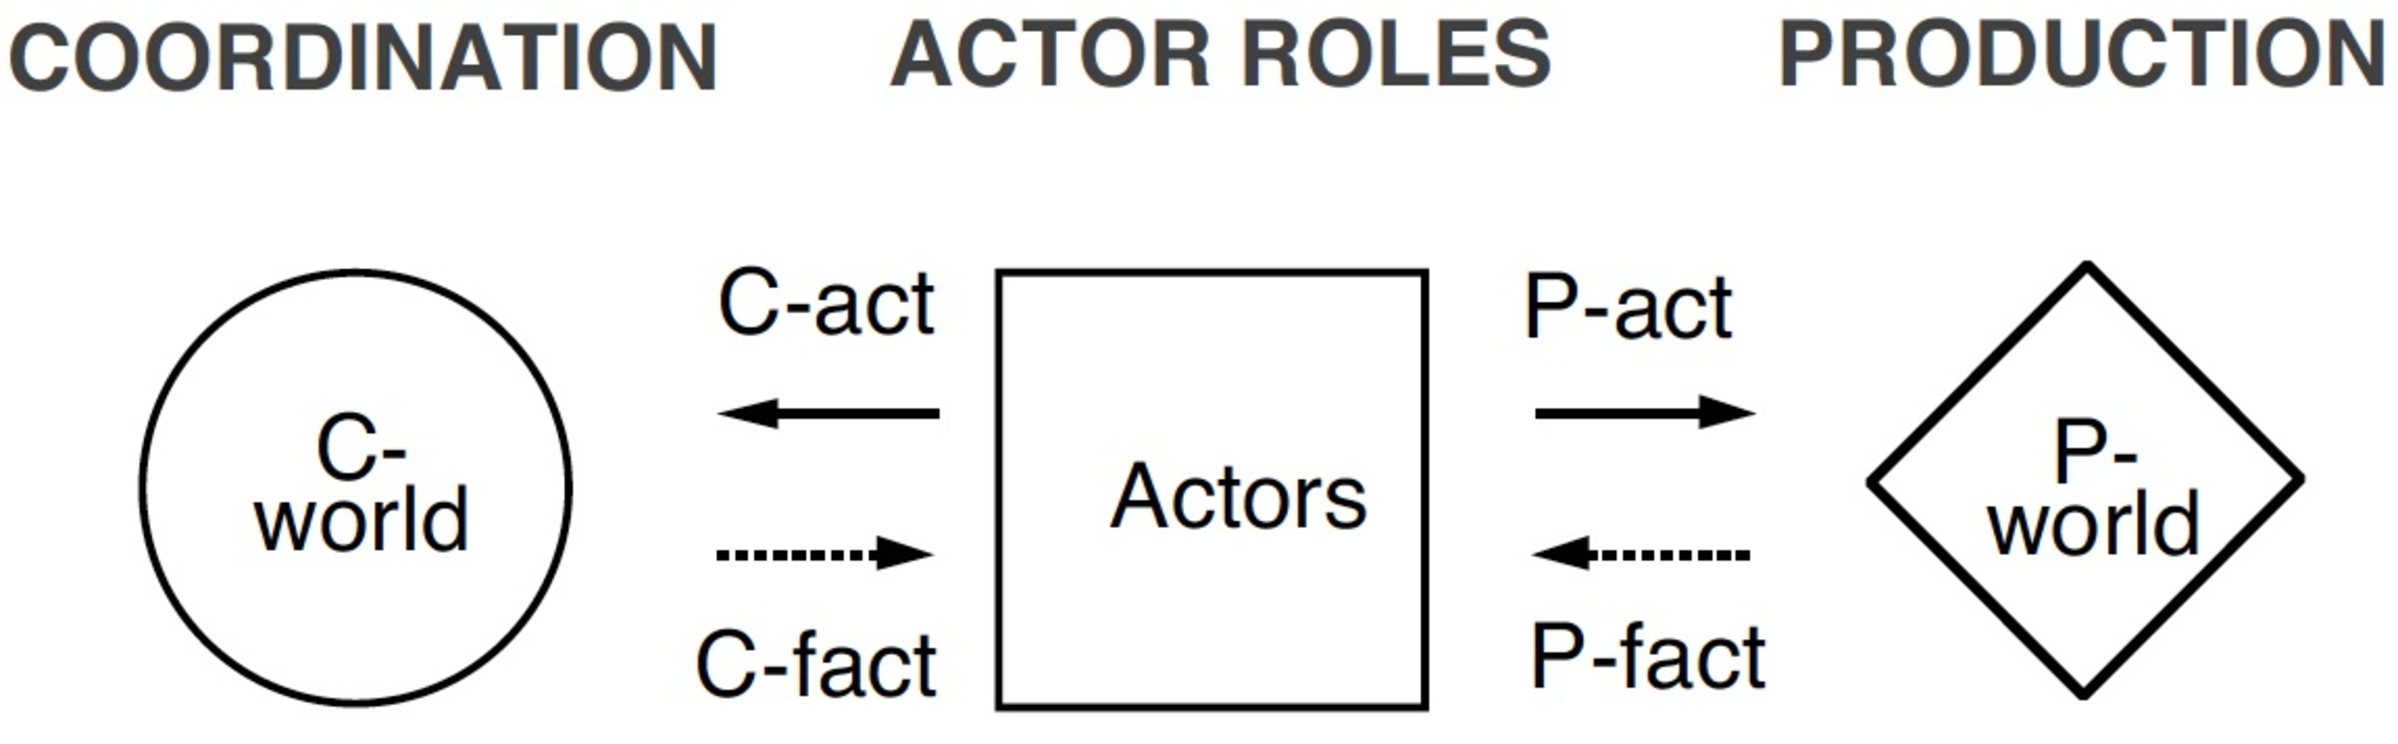
\includegraphics[scale=0.3]{obrazky/operation-axiom}}
\caption{Grafické znázornění operačního axiomu \cite{Dietz2006}}
\label{fig:operation_axiom}
\end{figure}
\end{center}

\subsubsection{C-acty}
C-acty probíhají mezi dvěma subjekty z nichž jeden se nazývá \textit{performer} a druhý \textit{adressee}. C-actů je několik typů, které můžeme rozdělit na intenční (\textit{intention}) a propoziční (\textit{proposition}).

Mezi příklady intenčních koordinačních činností řadíme:

\begin{itemize}
\item \textit{request}
\item \textit{promise}
\item \textit{question}
\item \textit{assertion}
\end{itemize}

V případě propozičních C-actů executor \uv{ohlašuje} P-fact a příslušný čas, kdy má být proveden.

\begin{center}
\begin{figure}[H]
\centerline{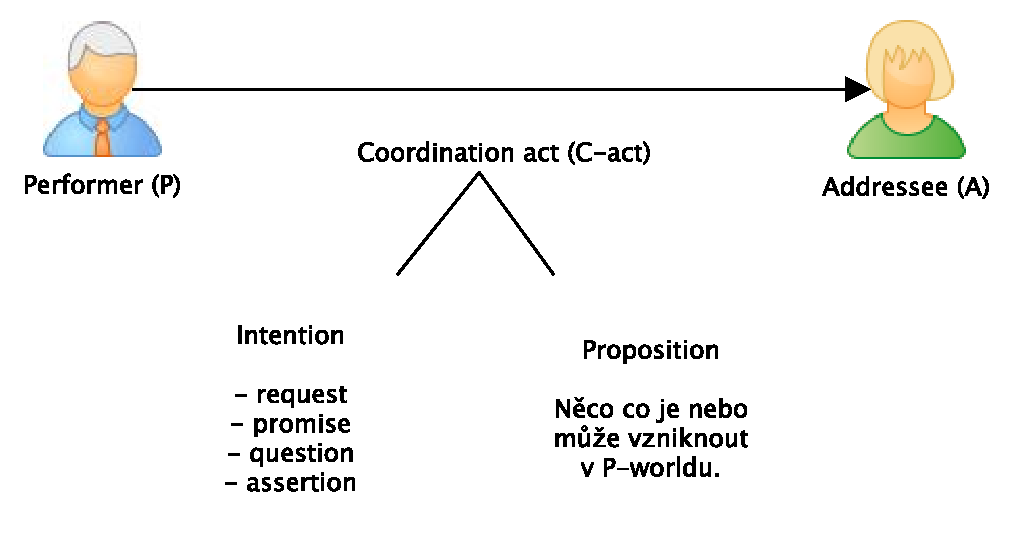
\includegraphics[scale=0.7]{obrazky/c-acts}}
\caption{Grafické znázornění C-actu \cite{Dietz2006}}
\label{fig:c-act}
\end{figure}
\end{center}

\subsubsection{P-facty}
Jak již bylo naznačeno, P-facty jsou buď hmotné nebo nehmotné. Zde je nezbytné poukázat na to, kdy tyto skutky začnou v P-worldu skutečně existovat. Před tím, než se to stane, je totiž nutné provést ještě dva C-facty a to \textit{state} a \textit{accept}. Teprve ve chvíli, kdy jsou tyto C-facty provedeny začíná P-fact skutečně existovat v P-worldu.

\subsubsection{Actoři}
\textit{Actoři} jsou aktivní subjekty uvnitř organizace. Jednají autonomně, tedy jejich činnost není vyvolána nějakou událostí \cite{Dietz2006}.  U actorů existují tři důležité vlastnosti, kterými jsou \textit{kompetence}, \textit{autorita} a \textit{zodpovědnost}.

Kompetencí je myšlena schopnost subjektu provádět P-acty a související C-acty. \cite{Dietz2006} uvádí příklad instalatéra, který má znalosti a zkušenosti, které jsou nezbytné pro to být profesionálním instalatérem.

Aby mohl být subjekt schopen vykonávat určitou profesi, musí pro to mít nějaký autoritativní základ, jako například být zaměstnancem určité organizace a podobně.

Subjekt je vázán normami, které se vztahují k řečené autoritě nebo k obecným normám platným ve společnosti, které očekávají, že bude svojí autoritu vykonávat odpovědným způsobem. V příkladu instalatéra to znamená, že se očekává, že bude jednat zodpovědně se svými zákazníky.

\subsection{Transakční axiom – The transaction axiom} \label{sec:transakcni_axiom}
\textit{Transakční axiom} dále rozebírá P-acty a C-acty a zejména to, jak spolu tyto činnosti souvisí. Základní myšlenkou transakčního axiomu, kterou formuluje \cite{Dietz2006}, je, že C-acty probíhají postupně za sebou ve stejných \textit{vzorech}. Tyto vzory se nazývají transakce a vždy zahrnují dva actory (initiator a executor) a jejich cílem je dosáhnout určitého výsledku, kterým je P-fact.

Každá transakce má tři fáze:

\begin{enumerate}
\item \textit{order phase},
\item \textit{execution phase},
\item \textit{result phase}.
\end{enumerate}

V rámci order phase se initiator a executor snaží dojít k \textit{dohodě} ohledně výsledku, kterého má být dosaženo (co, kdy). V execution phase je tento výsledek vytvořen a v result phase opět dochází k jednání mezi initiatorem a executorem, jestli vytvořený výsledek odpovídá požadavku initiatora.

Výsledek transakce (P-fact) začne existovat až ve chvíli, kdy je dokončena result phase, tedy když je P-fact schválen a přijat iniciátorem transakce. Do toho okamžiku P-fact v našem výkladu neexistuje.

Transakční vzory rozlišujeme dva: základní a standardní.

\subsubsection{Základní transakční vzor}
Základní transakční vzor je zjednodušený průběh transakce oproštěný od tzv. \textit{unhappy paths} neboli \uv{nešťastných scénářů}. Popisuje postup transakce v případě, kdy nenastanou žádné problémy, tedy executor vytvoří P-fact, který odpovídá požadavkům initiatora a tento P-fact je tedy bez komplikací akceptován.

Průběh zjednodušeného transakčního vzoru:

\begin{enumerate}
\item Initiator formuluje požadavek (\textit{request})
\item Executor učiní \textit{promise}
\item Executor provede požadavek (vytvoří P-fact) (\textit{execution})
\item Executor prohlásí výsledek za hotový (\textit{state})
\item Initiator akceptuje výsledek (\textit{accept})
\end{enumerate}

Základní transakční vzor je graficky znázorněn na obrázku \ref{fig:basic_transaction_pattern}.

\begin{center}
\begin{figure}[H]
\centerline{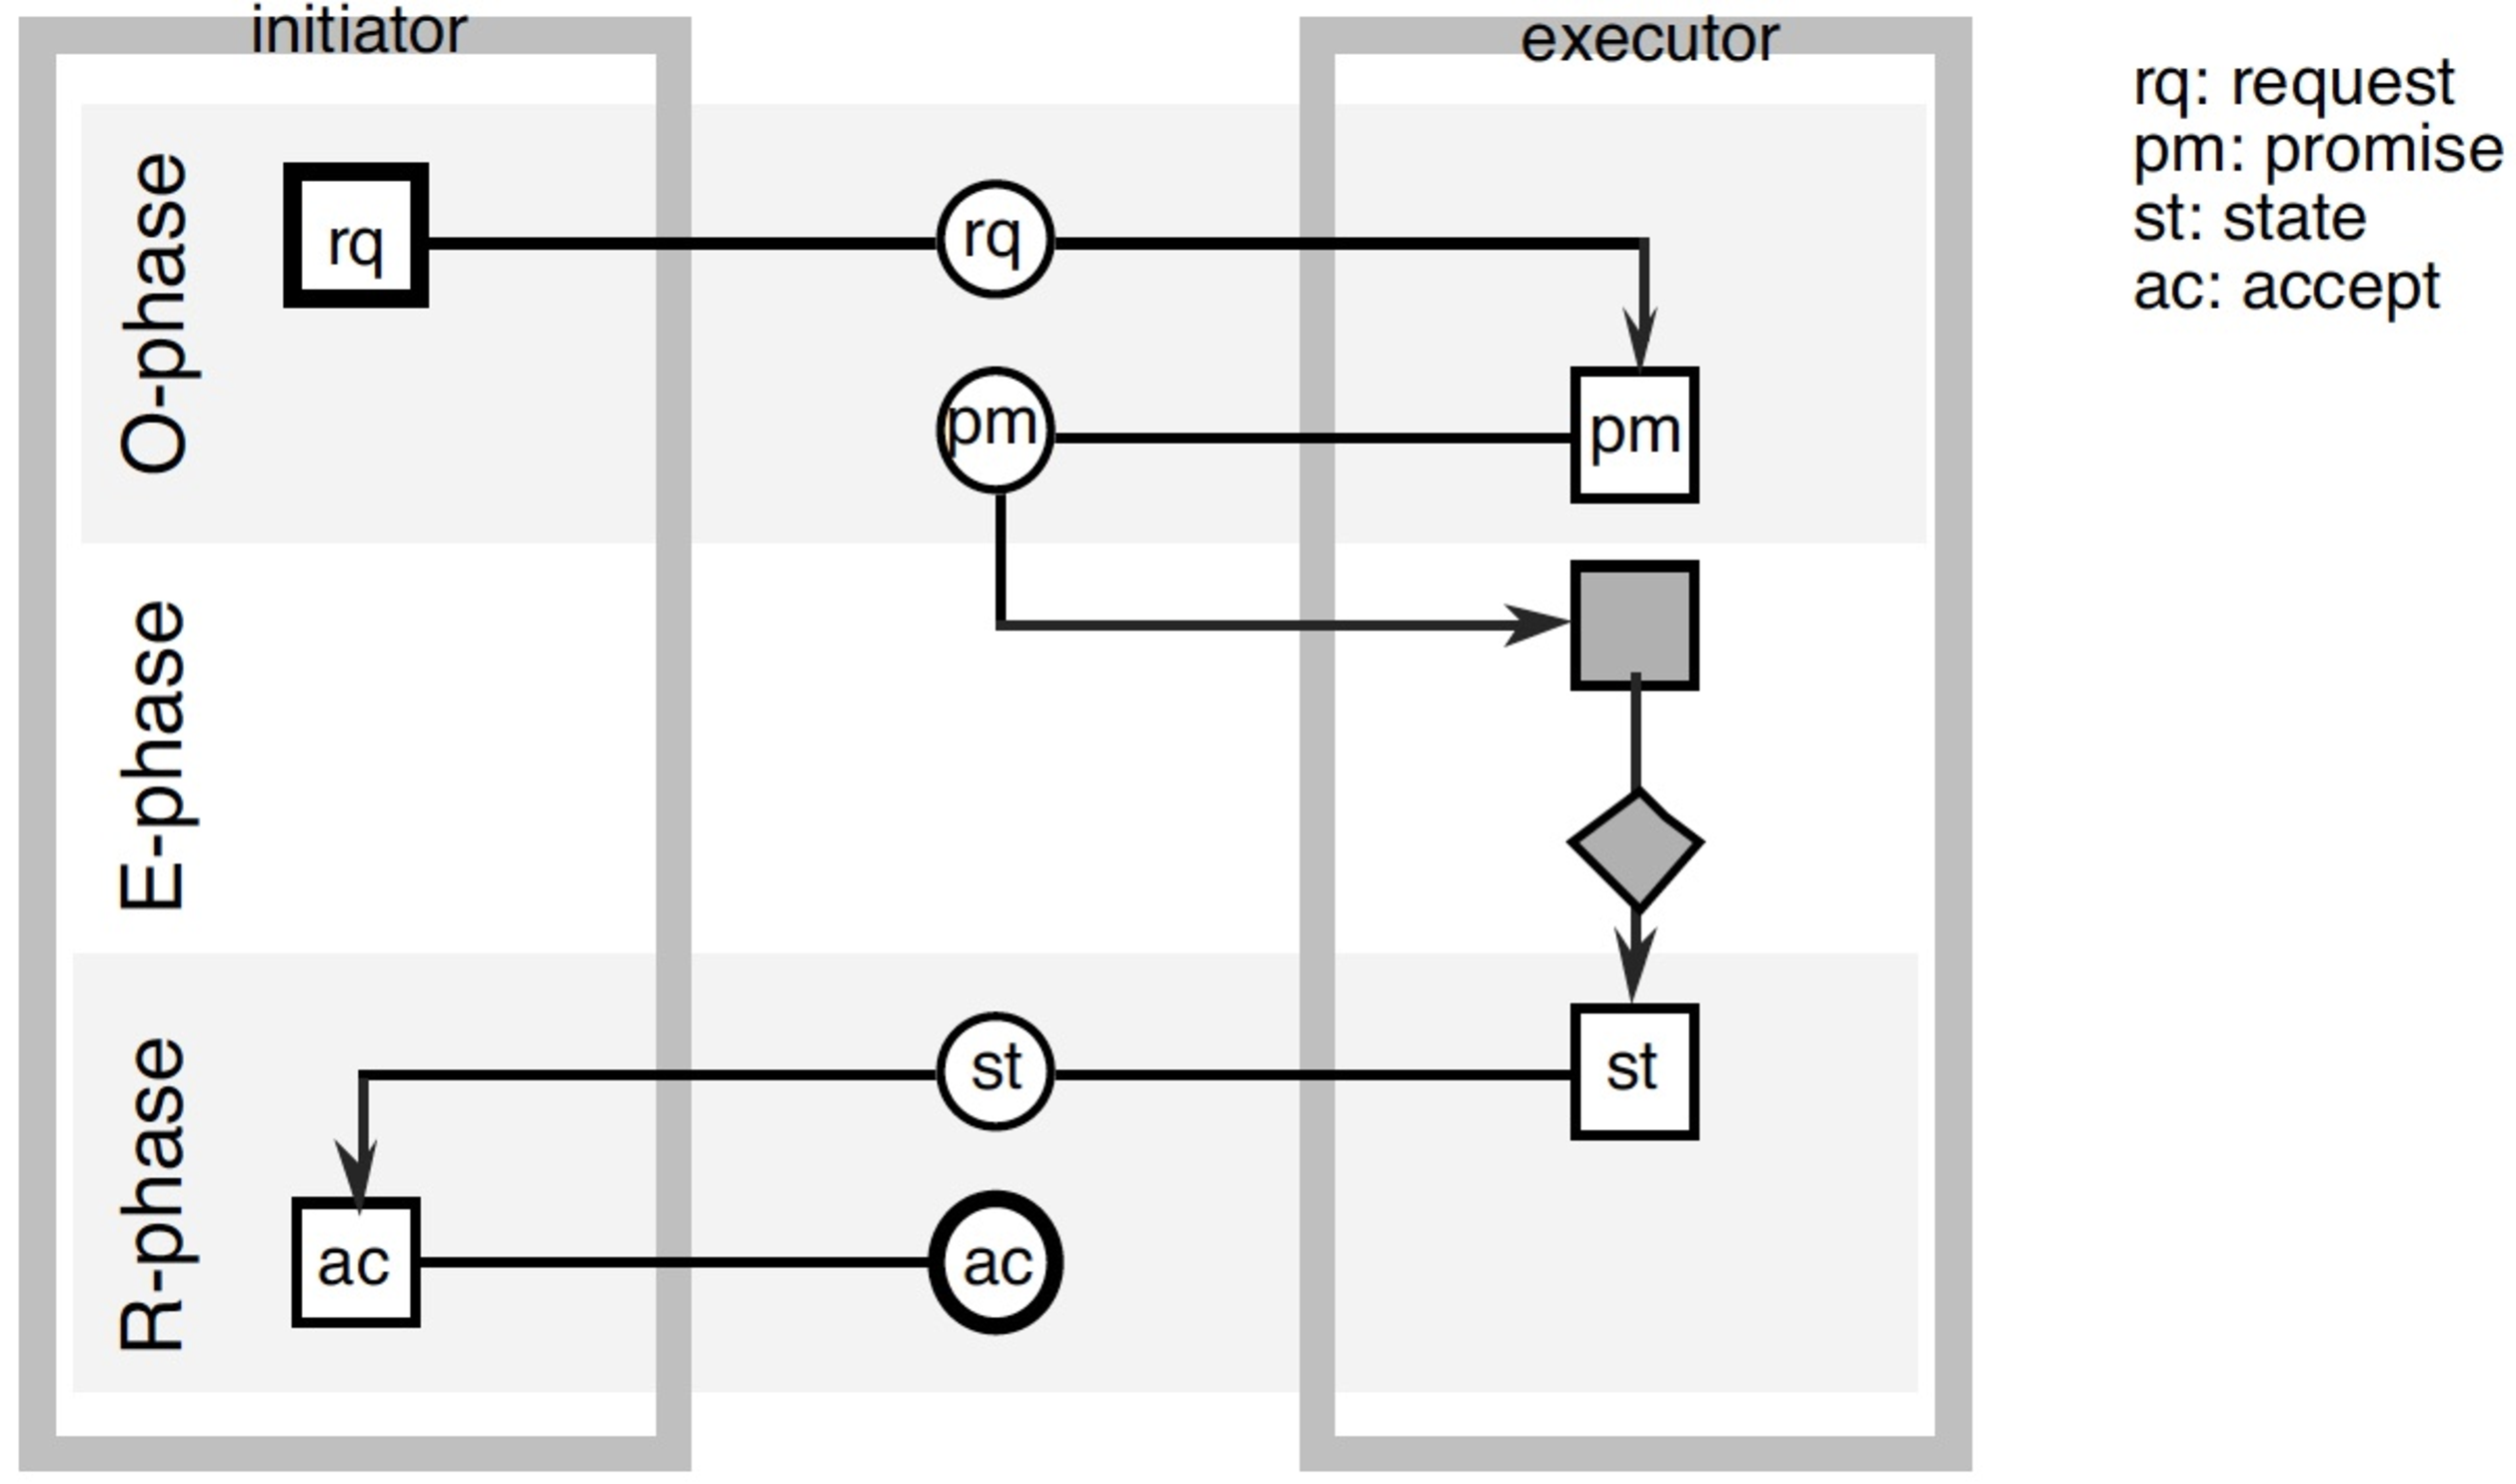
\includegraphics[scale=0.4]{obrazky/basic-transaction-pattern}}
\caption{Grafické znázornění základního transakčního vzoru \cite{Dietz2006}}
\label{fig:basic_transaction_pattern}
\end{figure}
\end{center}

\subsubsection{Standardní transakční vzor}
Standardní transakční vzor počítá i se situacemi, které v běžném životě neustále nastávají. Například se situací, kdy executor nemůže učinit \textit{promise} na požadavek iniciátora nebo initiator odmítne akceptovat výsledek transakce. Pokud toto nastane, dostává se celá transakce do tzv. \textit{diskusních stavů} (\textit{discussion states}), které mohou být buď \textit{nepřijmuto} (\textit{declined}) nebo \textit{odmítnuto} (\textit{rejected}).

Důvody pro odmítnutí \textit{požadavku} executorem vycházejí z těchto tří typů tvrzení (\textit{validity claims}):

\begin{itemize}
\item tvrzení pravdivosti (\textit{claim to truth}),
\item tvrzení oprávněnosti (\textit{claim to justice}),
\item tvrzení upřímnosti (\textit{claim to sincerity}).
\end{itemize}

\begin{center}
\begin{figure}[H]
\centerline{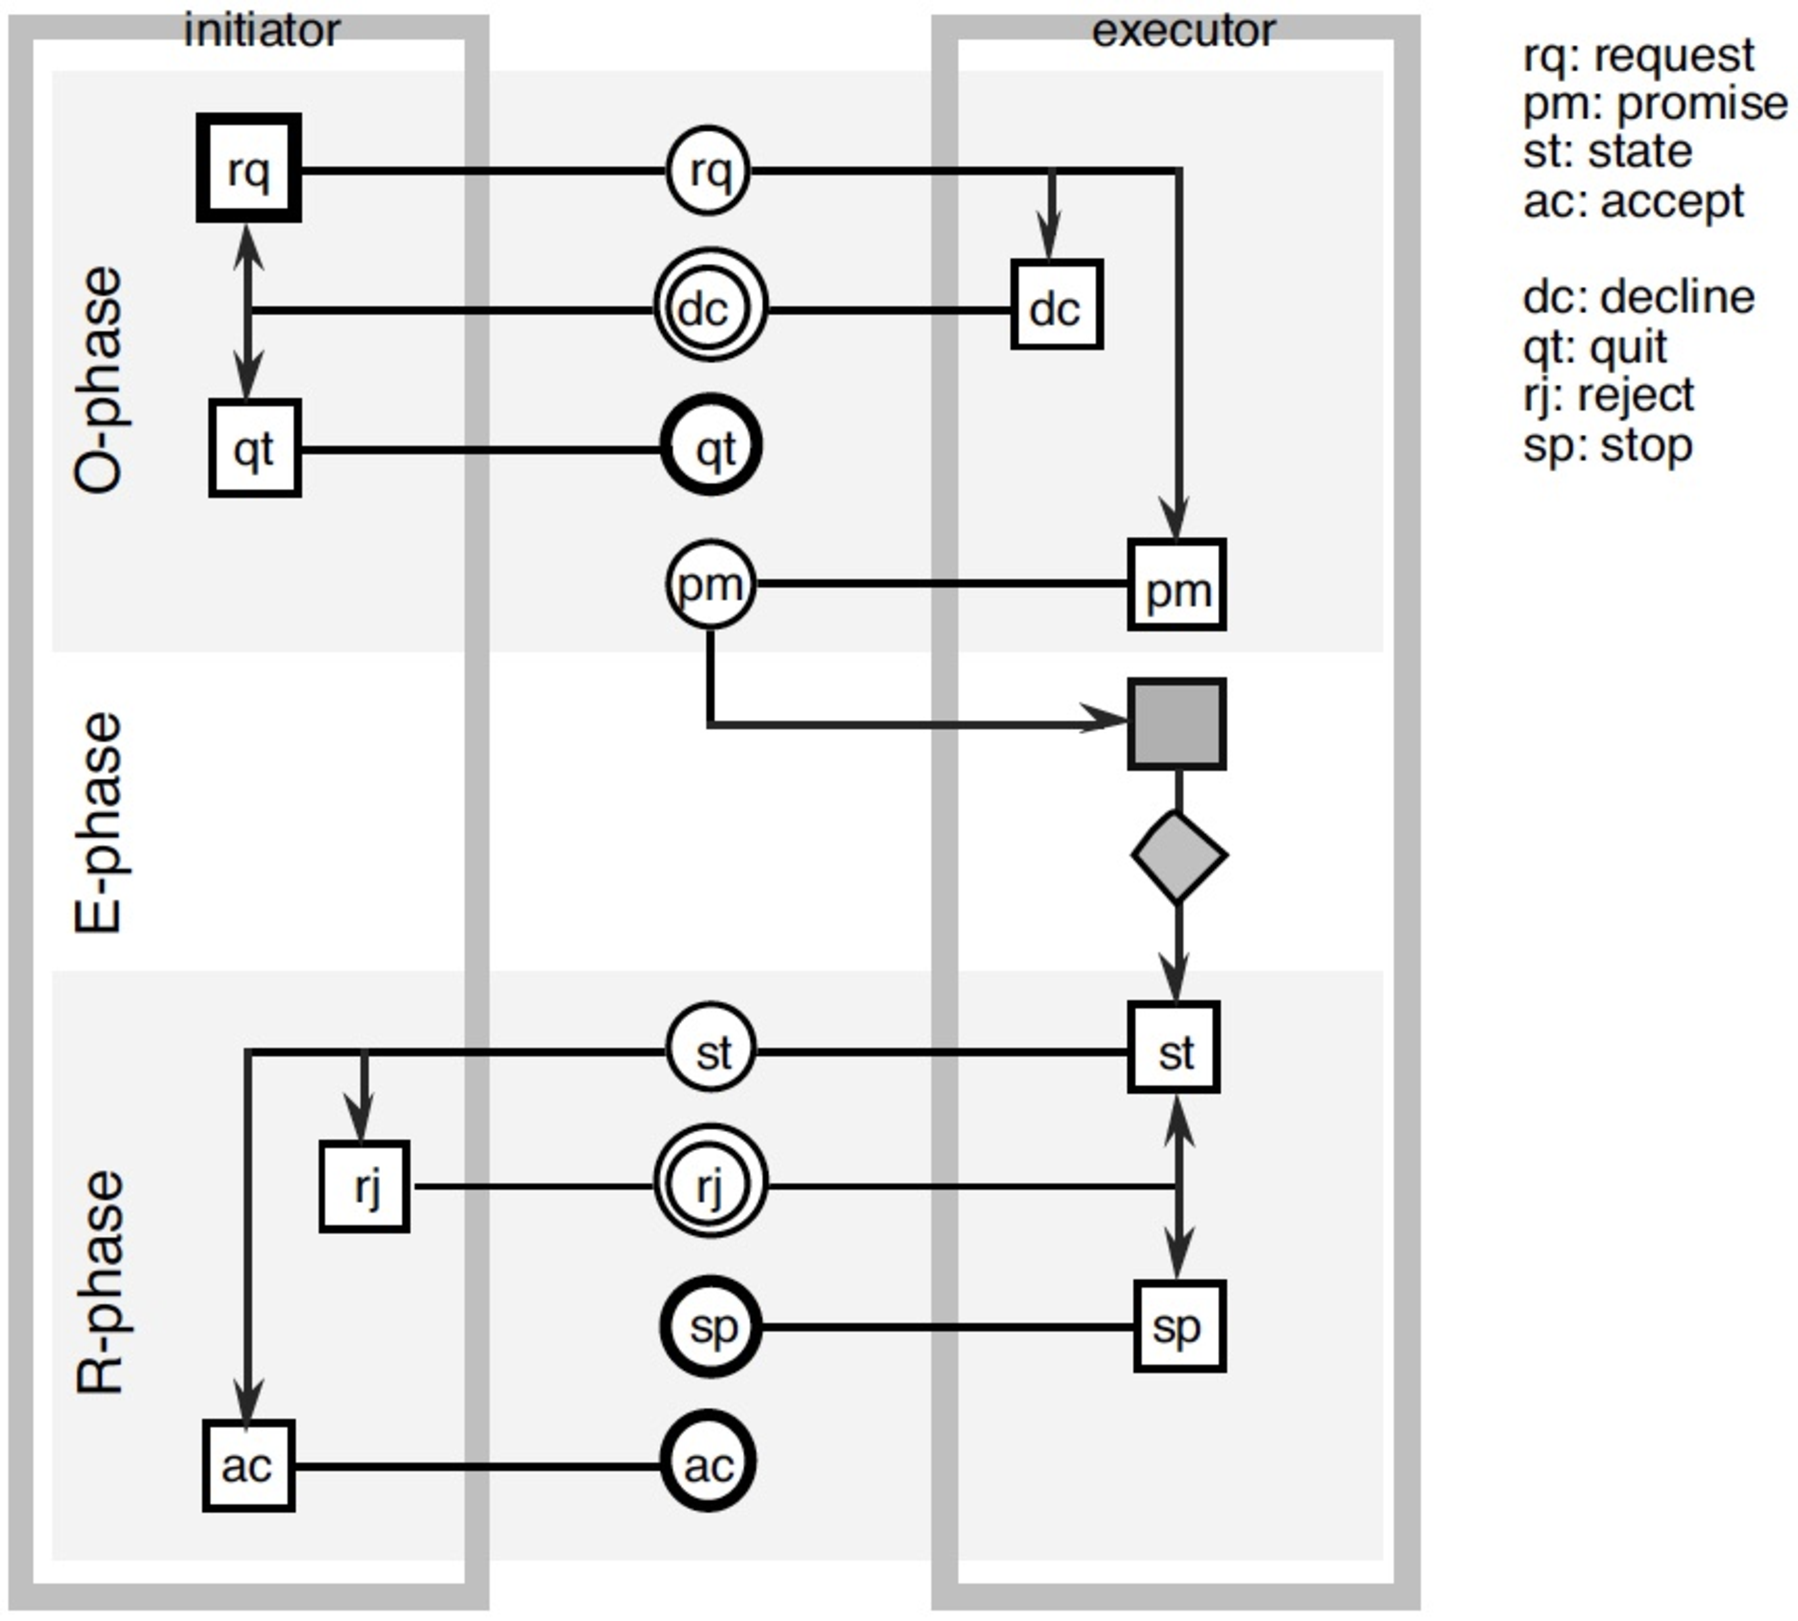
\includegraphics[scale=0.4]{obrazky/standard-transaction-pattern}}
\caption{Grafické znázornění standardního transakčního vzoru \cite{Dietz2006}}
\label{fig:standard_transaction_pattern}
\end{figure}
\end{center}

\subsubsection{Odvolávací vzory (Revoke patterns)}
V rámci standardního transakčního vzoru je možné odvolat kterýkoliv koordinační čin pomocí \textit{odvolávacího vzoru} pro daný C-act.

\subsection{Kompoziční axiom – The composition axiom} \label{sec:kompozicni_axiom}
Umět popsat strukturu konkrétní transakce je rozhodně přínosné, ale na ontologický popis organizace umět popsat jednotlivé transakce nestačí. Zde pak nastupuje \textit{kompoziční axiom}, který se zabývá tím, jak jsou jednotlivé transakce, respektive P-facty, propojené.

Kompoziční axiom tvrdí, že každá transakce je buď součástí jiné, je transakcí zákazníka organizace nebo je \textit{self-activated}. Logickou implikací tedy je, že transakce mohou obsahovat další transakce. \textit{Takto propojené transakce pak dohromady tvoří podnikový proces.}

Jak píše \cite{Dietz2006} kompoziční axiom je tak základem pro definici podnikového procesu, která říká, že podnikový proces je množina volně propojených transakcí. 

\subsection{Distinkční axiom – The distinction axiom} \label{sec:distinction_axiom}
Distinkční axiom tvrdí, že lidé mají tři různé typy schopností, které hrají roli v jejich chování.

\begin{itemize}
\item \textbf{forma} – jak už název napovídá, tato schopnost se týká formy v jaké jsou informace uchovávány, předávány, přijímány atd.
\item \textbf{informa} – v tomto případě jde o obsah informace a její komunikaci mezi lidmi a plně abstrahujeme od formy v jaké je informace komunikována.
\item \textbf{performa} – jedná se o nejvyšší formu lidských schopností. Jde zde o vytváření nových originálních věcí přímo nebo nepřímo pomocí komunikace. To se týká závazků, rozhodnutí, posuzování apod.
\end{itemize}

Jak píše \cite{Vejrazkova2013}, pro jeden infologický čin (performa) musíme provést více infologických činů (informa) a pro jeden infologický čin musíme provést více datalogických činů (forma). Toto rozlišení umožňuje výrazně zjednodušit procesní modely, protože se při jejich tvorbě zabýváme pouze ontologickými činy.

\section{Teorém organizace – The organization theorem}

V předchozí sekci jsou popsány čtyří axiomy \ptheory{}, které přináší z různých úhlů pohled na chod organizace, její operace a uspořádání. Tyto pojmy však samy o sobě nestačí k vytvoření ontologického modelu, který bude výstižný, úplný, ucelený a konzistentní. Teorém organizace se zabývá právě tím.

Dle teorému organizace je každá organizace strukturovaná jako heterogenní systém, který je tvořen třemi vrstvami, z nichž každá představuje jeden homogenní systém: \cite{Dietz2006}

\begin{itemize}
\item B-organizace (B=Business)
\item I-organizace (I=Intellect)
\item D-organizace (D=Document)
\end{itemize}

Mezi těmito vrstvami (systémy) existuje velká provázanost. D-organizace podporuje I-organizaci a I-organizace podporuje B-organizaci. Provázanost mezi těmito systémy zajišťuje člověk. U tohoto konstatování je třeba se zastavit. Rozdělení organizace do tří systému si není možné představovat tak, že existují v organizaci nějaká B-oddělení, I-oddělení nebo D-oddělení nebo dokonce B-lidé, I-lidé či D-lidé. Naopak v realitě nic takového neexistuje. Lidé i skupiny lidí zastávají role ve všech systémech najednou a volně mezi nimi \uv{přechází}.

Rozdíl mezi jednotlivými systémy tvoří jejich výstupy. Jak uvádí \cite{Dietz2006} výstup B-organizace je ontologický, výstup I-organizace je infologický a výstup D-organizace je datalogický.

\begin{center}
\begin{figure}[H]
\centerline{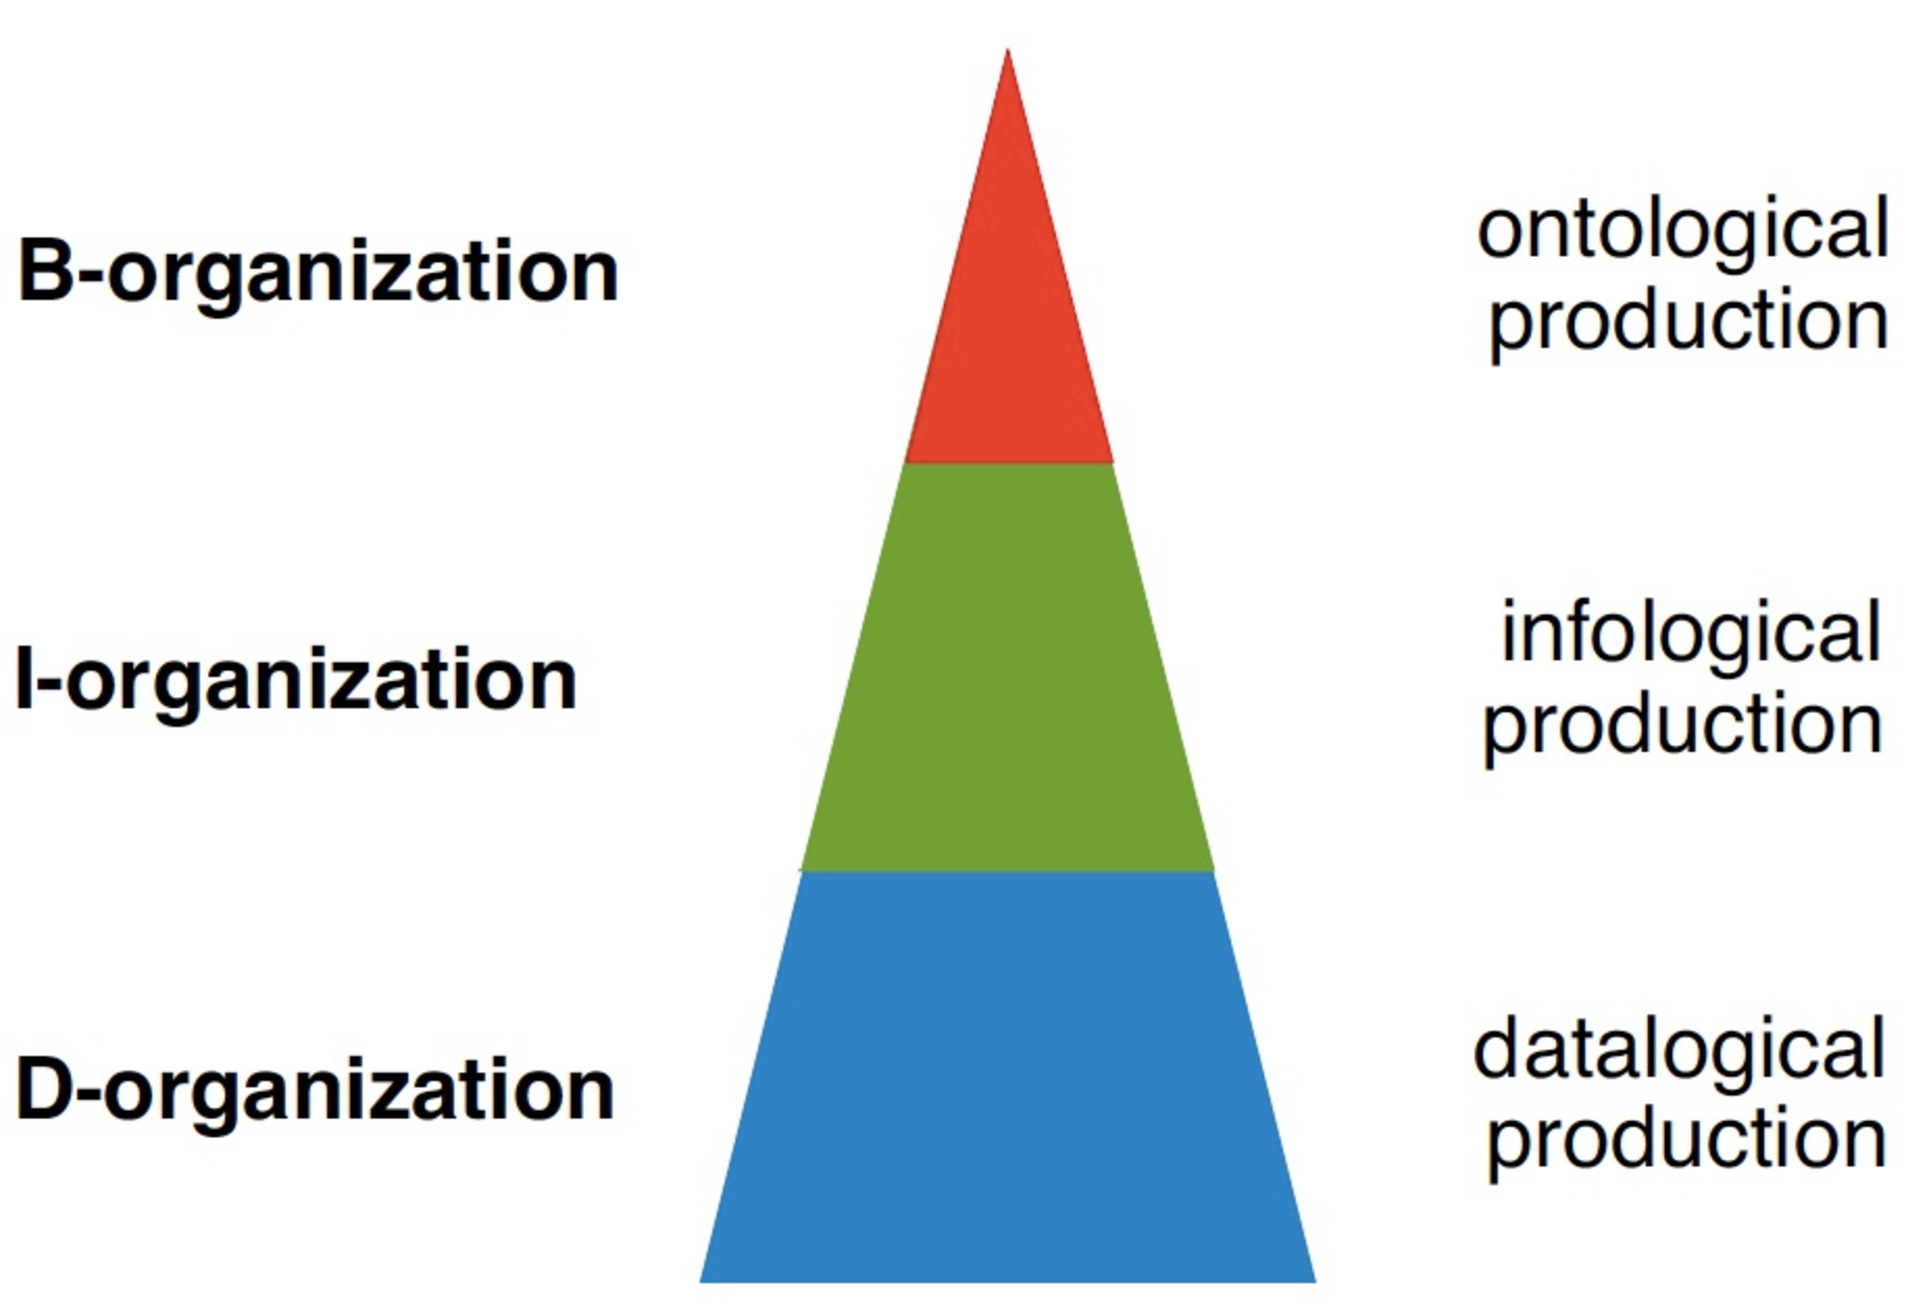
\includegraphics[scale=0.3]{obrazky/organization-theorem}}
\caption{Grafické znázornění organizačního teorému \cite{Dietz2006}}
\label{fig:oraganization_theorem}
\end{figure}
\end{center}

Na vrcholu této pyramidy je B-organizace neboli ontologický level. Tím je naznačeno, že porozumění chodu organizace na této úrovni je kompletní, tedy není z něj nic vynecháno.

Pro lepší pochopení provázanosti jednotlivých systémů v organizaci bude nyní jejich provázanost hlouběji rozebrána. I-organizace poskytuje \uv{informační zdroje} pro fungování B-organizace. \cite{Dietz2006} uvádí příklad s výpočtem denního obratu, který B-actor v B-organizaci chce vytvořit. Za tímto účelem je ale nejprve v I-organizaci I-actorem třeba provést několik jasně definovaných výpočtů (I-transakce) a následně doručit B-actorovi výsledek, kterým je právě denní obrat.

Dále je nutné rozebrat propojení mezi I-organizací a I-actorem s D-organizaci a D-actorem. V příkladu počítání denního obratu musí nejdříve I-actor sčítající jednotlivé položky, které denní obrat tvoří, někde tyto položky (čísla) opatřit. Tyto údaje získá samozřejmě v D-organizaci pomocí D-transakcí.

Jak už bylo naznačeno výše, není důležité, jestli v tomto konkrétním případě je B-actor, I-actor a D-actor několik osob nebo jeden člověk a stejně tak B-organizace, I-organizace či C-organizace mohou být na několika kontinentech nebo uvnitř jedné kanceláře.

\section{Základní modely DEMO}
V této sekci bude rozebrána vlastní metodologie DEMO. Rozebrány budou zejména dvě věci: typy modelů, ze kterých se DEMO skládá a doporučený postup, jak v DEMO modelovat. Přesný popis jednotlivých elementů je možné dohledat například v \cite{Dietz2006}.

Jak píše \cite{Vejrazkova2012}, základními elementy DEMO jsou \textit{ontologické transakce} a \textit{actoři}.

\subsection{Ontologická transakce}
Ontologické transakce jsou transakce, jejichž výsledkem je vytvoření něčeho nového, ať už se jedná o věc hmotnou či nehmotnou. Jak už uvádí distinkční axiom \ptheory{}, který byl popsán výše, ontologické transakce probíhají na ontologické úrovni (performa).

\subsection{Actor}
Každá transakce má vždy jednoho initiatora a jednoho executora.

\subsection{Modely DEMO (Aspect models)}
Struktura a popis jednotlivých modelů vychází zejména z \cite{Vejrazkova2012} a \cite{Dietz2005}.

Jak už bylo zevrubně popsáno v kapitole \ref{chap:2}, DEMO se skládá ze 4 hlavních modelů a dalších podmodelů. Jedná se o:

\begin{itemize}
\item Construction Model (CM)
\item Process Model (PM)
\item State Model (SM)
\item Action Model (AM)
\end{itemize}

Každý z těchto modelů se pohybuje na jiné úrovni abstrakce, což se dá dobře popsat na principu pyramidy, který je naznačen na obrázku \ref{fig:aspect_model}.
Construction Model, který je usazen na vrcholu této pyramidy pracuje s nejvyšší úrovní abstrakce a naopak Action Model, který je na obrázku zobrazen při základu pyramidy je už velmi podrobný a detailní. Všechny tyto modely dohromady tvoří kompletní ontologickou znalost organizace.

\begin{center}
\begin{figure}[H]
\centerline{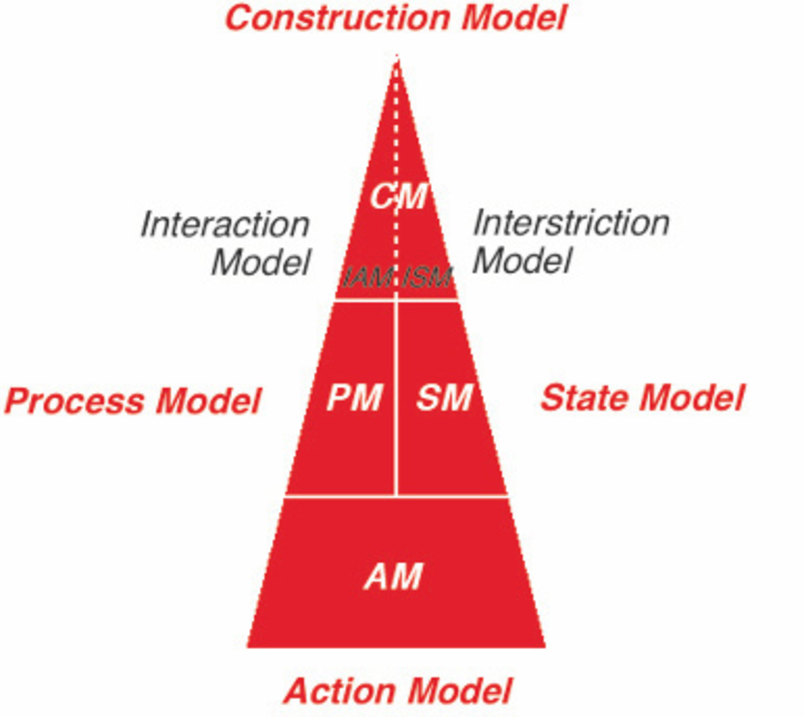
\includegraphics[scale=0.75]{obrazky/aspect-models}}
\caption{DEMO Aspect models \cite{Dietz2006}}
\label{fig:aspect_model}
\end{figure}
\end{center}

\subsubsection{Construction Model}
Jak už jeho název napovídá, Construction Model se zabývá konstrukcí organizace na té nejvyšší úrovni abstrakce. Construction Model tvoří dva podmodely: \textit{Interaction Model (IAM)} a \textit{Interstriction Model (ISM)}. Cílem Construction Modelu je v podstatě jen identifikovat jednotlivé ontologické transakce a jejich výsledky. 


Interaction Model (IAM) zobrazuje actory (initiatory a executory) a transakce, které tito actoři vykonávají. Jedná se o vysoce abstraktní pohled, takže v něm není vidět jednotlivé kroky transakcí, ale čistě jen interakci mezi actory, která je prováděna právě prostřednictvím transakce.

IAM se skládá z \textit{Transaction Result Table (TRT)} a \textit{Actor-Transaction Diagramu (ATD)}. TRT je jednoduchá tabulka identifikovaných ontologických transakcí a jejich výsledků. ATD je diagram, který ukazuje transakce mezi actory.

ISM je založen na IAM a obsahuje dva diagramy a tabulku:

\begin{itemize}
\item \textbf{Actor Bank Diagram (ABD)} – zobrazuje vztah mezi actory a informačními bankami
\item \textbf{Organization Construction Diagram (OCD)} – jedná se o kombinaci ABD s ATD. Tedy actoři, transakce mezi nimi a navíc ještě propojení s informačními bankami.
\item \textbf{Bank Contents Table (BCT)} – tabulka popisující obsah bank faktů.
\end{itemize}

\subsubsection{Process Model (PM)}
Pokud se Construction Model nacházel na vysoké úrovni abstrakce, tak \textit{Process Model (PM)} jde o krok více do detailu. Kde CM pouze pojmenovával transakce, PM rozvádí jejich jednotlivé kroky tak, jak jsou popsány v transakčním axiomu \ptheory{}. Zároveň ukazuje také vztahy mezi jednotlivými transakcemi. Stále je však potřeba mít na paměti, že ačkoliv PM detailně popisuje strukturu podnikového procesu, tak je stále abstrahován od implementace a vlastní realizace daného procesu včetně takových věcí jako je výměna dat apod.

V případě přípravy na vývoj informačního systému je PM dobré místo, odkud začít se soupisem požadavků a případů užití.


PM se skládá z:

\begin{itemize}
\item \textbf{Process Structure Diagram (PSD)} – jak už název napovídá, zobrazuje strukturu procesu. Jak už bylo popsáno výše, podnikový proces se skládá z jedné či více vzájemně provázaných transakcí. Kroky, které nejsou popsány v PSD nejsou povolené a PSD by měl obsahovat i odvolávací vzory.
\item \textbf{Information Use Table (IUT)} – přímo se váže na State Model. Pro každou objektovou třídu, typ skutku a výsledku ze State Modelu specifikuje, v jakých krocích PM se používají jejich instance. 
\end{itemize}

\subsubsection{State Model (SM)}
\textit{State Model (SM)} se zabývá především P-worldem – jeho objektovými třídami, typy skutků, typy výsledků a existenčními ontologickými pravidly. SM je přímo navázaný na Action Model, zobrazuje ale pouze informace, které jsou relevantní pro chod organizace. SM obsahuje:

\begin{itemize}
\item \textbf{Object Fact Diagram (OFD)} – tento diagram zobrazuje vztah mezi objektovými třídami a typy výsledků.
\item \textbf{Object Property List (OPL)} – popisuje objektové třídy a jejich vlastnosti.
\end{itemize}

\subsubsection{Action Model (AM)}
\textit{Action Model (AM)} existuje v metodologii DEMO na té nejnižší úrovni abstrakce a tudíž je velmi detailní a ostatní modely na něm stojí, AM popisuje především pravidla, kterými se operace v organizaci řídí. Tato pravidla jsou v AM popsána slovně pomocí pseudo-algoritmického jazyka, ve kterém specifikují co má být uděláno při request, promise, state a accept.

Už z popisu výše je zřejmé, že AM bude velmi užitečný nástroj při implementaci softwaru. Action Model je ontologicky atomický, což znamená, že již nemůže být dále rozdělen na podmodely.

\section{Postup při tvorbě DEMO modelů}
\cite{Dietz2006} přímo nespecifikuje, jak a v jakém pořadí modely vytvářet. Pro zápis postupu v této sekci je proto využit a doplněn postup uvedený v \cite{Vejrazkova2012}.

\begin{enumerate}
\item Prvním krokem při tvorbě DEMO modelů je získání textového popisu organizace nebo procesu. Textový popis lze získat od doménových a procesních vlastníků.
\item Na textový popis je aplikována \textit{Performa-Informa-Forma analýza} a jednotlivé aktivity v popisu jsou klasifikovány jako ontologické, infologické nebo datalogické.
\item V označených aktivitách jsou rozlišeny C-acty a P-acty a dále actoři, kteří jsou za jejich provedení zodpovědní.
\item Vytvoření \textit{Transaction Result Table (TRT)} obsahující všechny identifikované transakce, jejich výsledky a transakční kroky identifikované v předchozím kroku.
\item Aplikace kompozičního axiomu a zápis struktury výsledků transakcí dle závislostí, které je možné odhalit v textovém popisu.
\item Identifikace rolí actorů pro každou transakci (Actor-Initiator, Actor-Executor).
\item Rozhodnutí, které transakce patří dovnitř organizace, a které probíhají vně. Vytvoření \textit{Actor-Transaction Diagramu (ATD)}. Nyní máme k dispozici kompletní \textit{Interaction Model (IAM)}.
\item Vytvoření \textit{Process Structure Diagramu (PSD)}, čímž jsme vytvořili \textit{Process Model (PM)}.
\item Na základě textového popisu je možné identifikovat všechny \textit{action rules} a vytvořit na jejich základně \textit{Action Model (AM)}.
\item Díky AM a provedení analýzy tříd objektů a typů vlastností je možné vytvořit \textit{Object Fact Diagram (OFD)} a \textit{Object Property List (OPL)} ze \textit{State Modelu (SM)}, který tímto vytvoříme.
\item Nyní je možné vytvořit poslední část PM, kterou je \textit{Information Use Table (IUT)}.
\item Na závěr je nutné identifikovat toky informací a na jejich základě a IAM je možné vytvořit \textit{Actor Bank Diagram (ABD)}, \textit{Organization Construction Diagram (OCD)} a \textit{Bank Contents Table (BCT)}. Po dokončení tohoto kroku máme k dispozici i \textit{Interstriction Model (ISM)}..
\end{enumerate}